\subsection{Mission Operation }
HurriSat is designated to cover ground area of 100,000 square miles as in Figure \ref{fig:coverage}. The target area is highlighted in neon blue ticker from STK \cite{AGISolutions2021} simulation. Now if there is any possible high or low wind  formation present in the targeted area (see possible\_formation point in the map),  it is first picked up by the spectral camera we have, and is logged by the on board computer processor. Once the image is processed and if indeed there's a high wind formation at the target area; the ground station is signaled, and heat signatures picked up by the infrared camera is transmitted.The cubesat then adjusts it self via its ADCS navigation system. This is where the narrow camera gets triggered to  actively follow the hurricane. It's purpose is to narrowly focus on target area 2 (see highlighted in green) and taking detailed images of 10m/pixel or less for possible hurricane size, relative speed, and impact area. A typical hurricane will travel across the ocean at a speed of about 250 miles (400 kilometers) per day, or about 10 to 15 miles (16 to 24 kilometers) per hour \cite{Sumanth2019}. Thus, for an area of that size HurriSat is able to pick it up all in one bypass without having to use any thrust.  Should the hurricane linger or move faster than expected (which is highly unlikely),  HurriSat can get an update after making 15-20 min orbital journey seen in Figure \ref{fig:orbi}. This map shows the actual operation orbit for HurriSat using STK.  It's inclined at 35 degree, at 800km to get a more closer and detailed view of hurricane sizes. This also helps reduce any signal loss from the ISIS antenna, whilst updating to ground station every now and then.
\FloatBarrier
\begin{figure}[hbt!]
    \centering
    \subfloat[Ground Coverage]{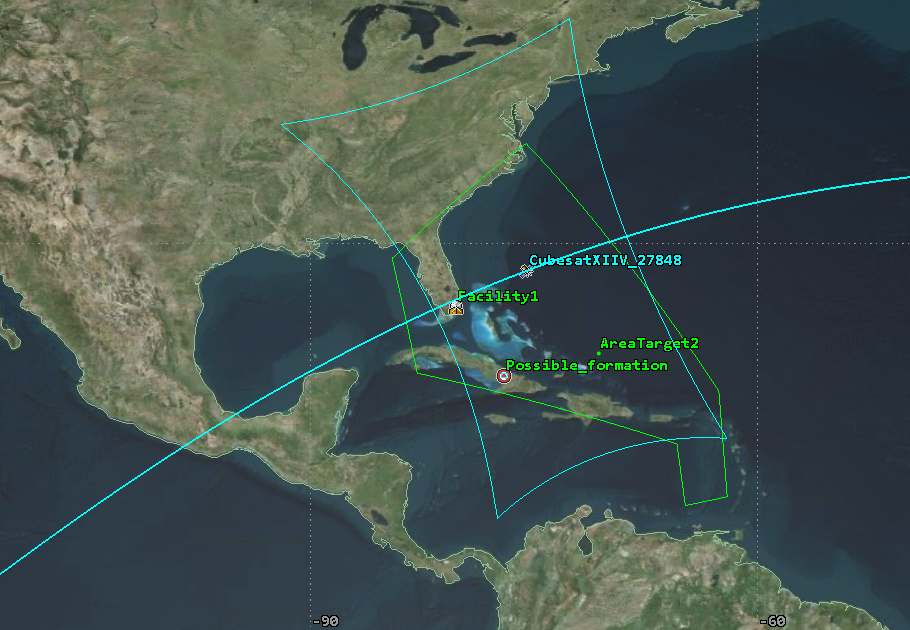
\includegraphics[width=7cm,height=5cm]{Images/flatmap.PNG}\label{fig:coverage}}\hspace{2mm}
    \subfloat[HurriSat Orbit]{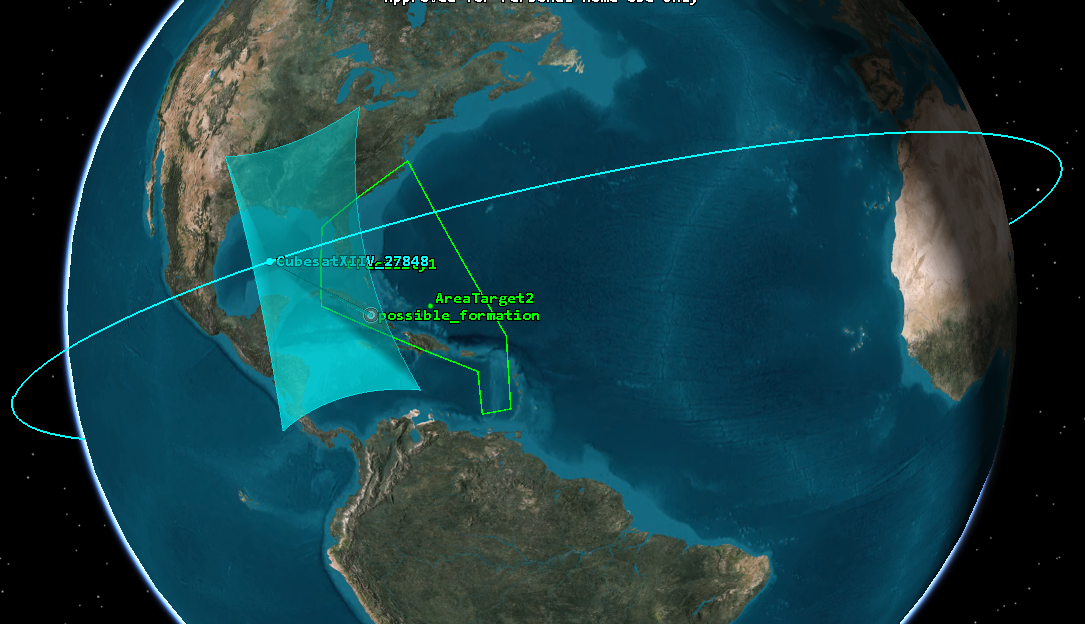
\includegraphics[width=7cm,height=5cm]{Images/satpic.PNG}\label{fig:orbi}}
    \caption{HurriSat Orbit and Ground Coverage}
    \label{fig:orbiGC}
\end{figure}
%\begin{figure}[hbt!]
%    \centering
%    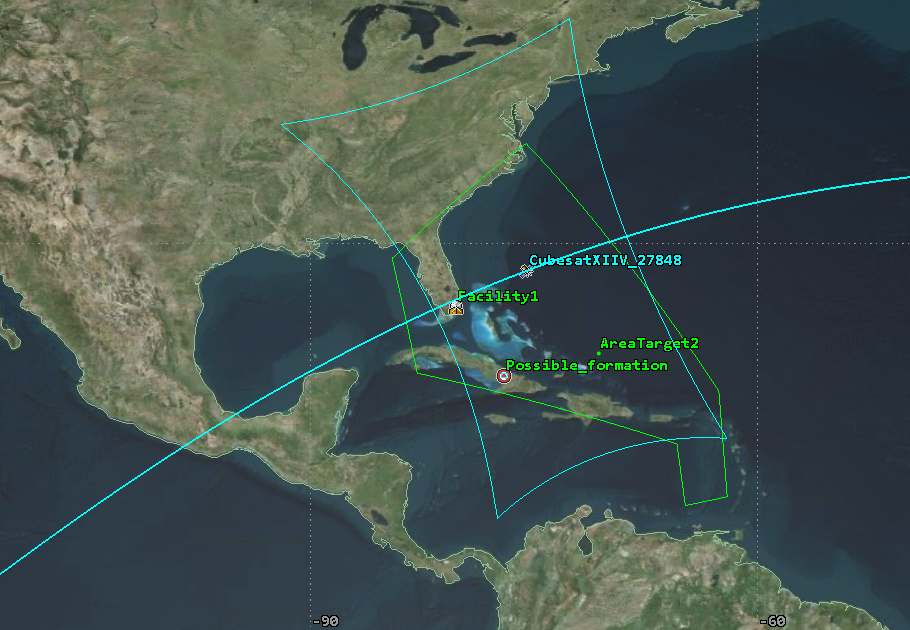
\includegraphics[width=\textwidth,frame, scale=0.6, keepaspectratio]{Images/flatmap.PNG}
%    \caption{Ground Coverage}
%    \label{fig:coverage}
%\end{figure}
\\
%\begin{figure}[hbt!]
%    \centering
%    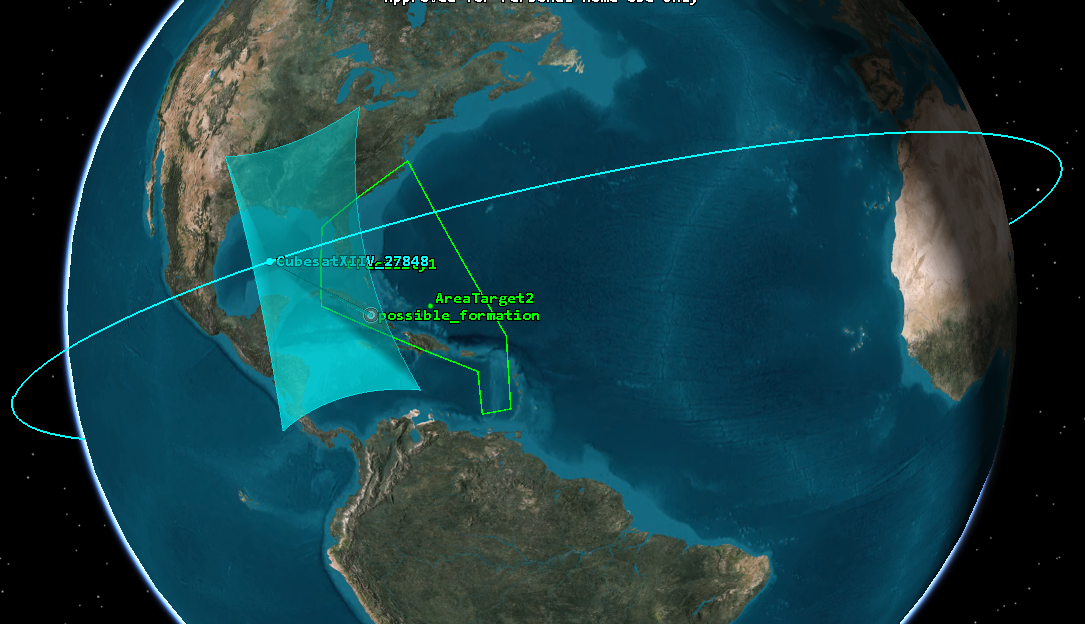
\includegraphics[width=\textwidth,frame, scale=0.6, keepaspectratio]{Images/satpic.PNG}
%    \caption{HurriSat Orbit}
%    \label{fig:orbi}
%\end{figure}\\
\FloatBarrier
\subsection{Mission Architecture}
Figure \ref{fig:march} is the overall mission architecture diagram. This diagram shows a high-level summary of the HurriSat project relative to its purpose and mission life. For easier exploration we have divided it into four main phases. The pre-launch, launch, post-launch, and end of life. Light blue blocks in the diagram outlines who or what entity will be involved, and the light red circle blocks indicate the ultimate mission (goal) for each section. \\

\begin{figure}[hbt!]
    \centering
    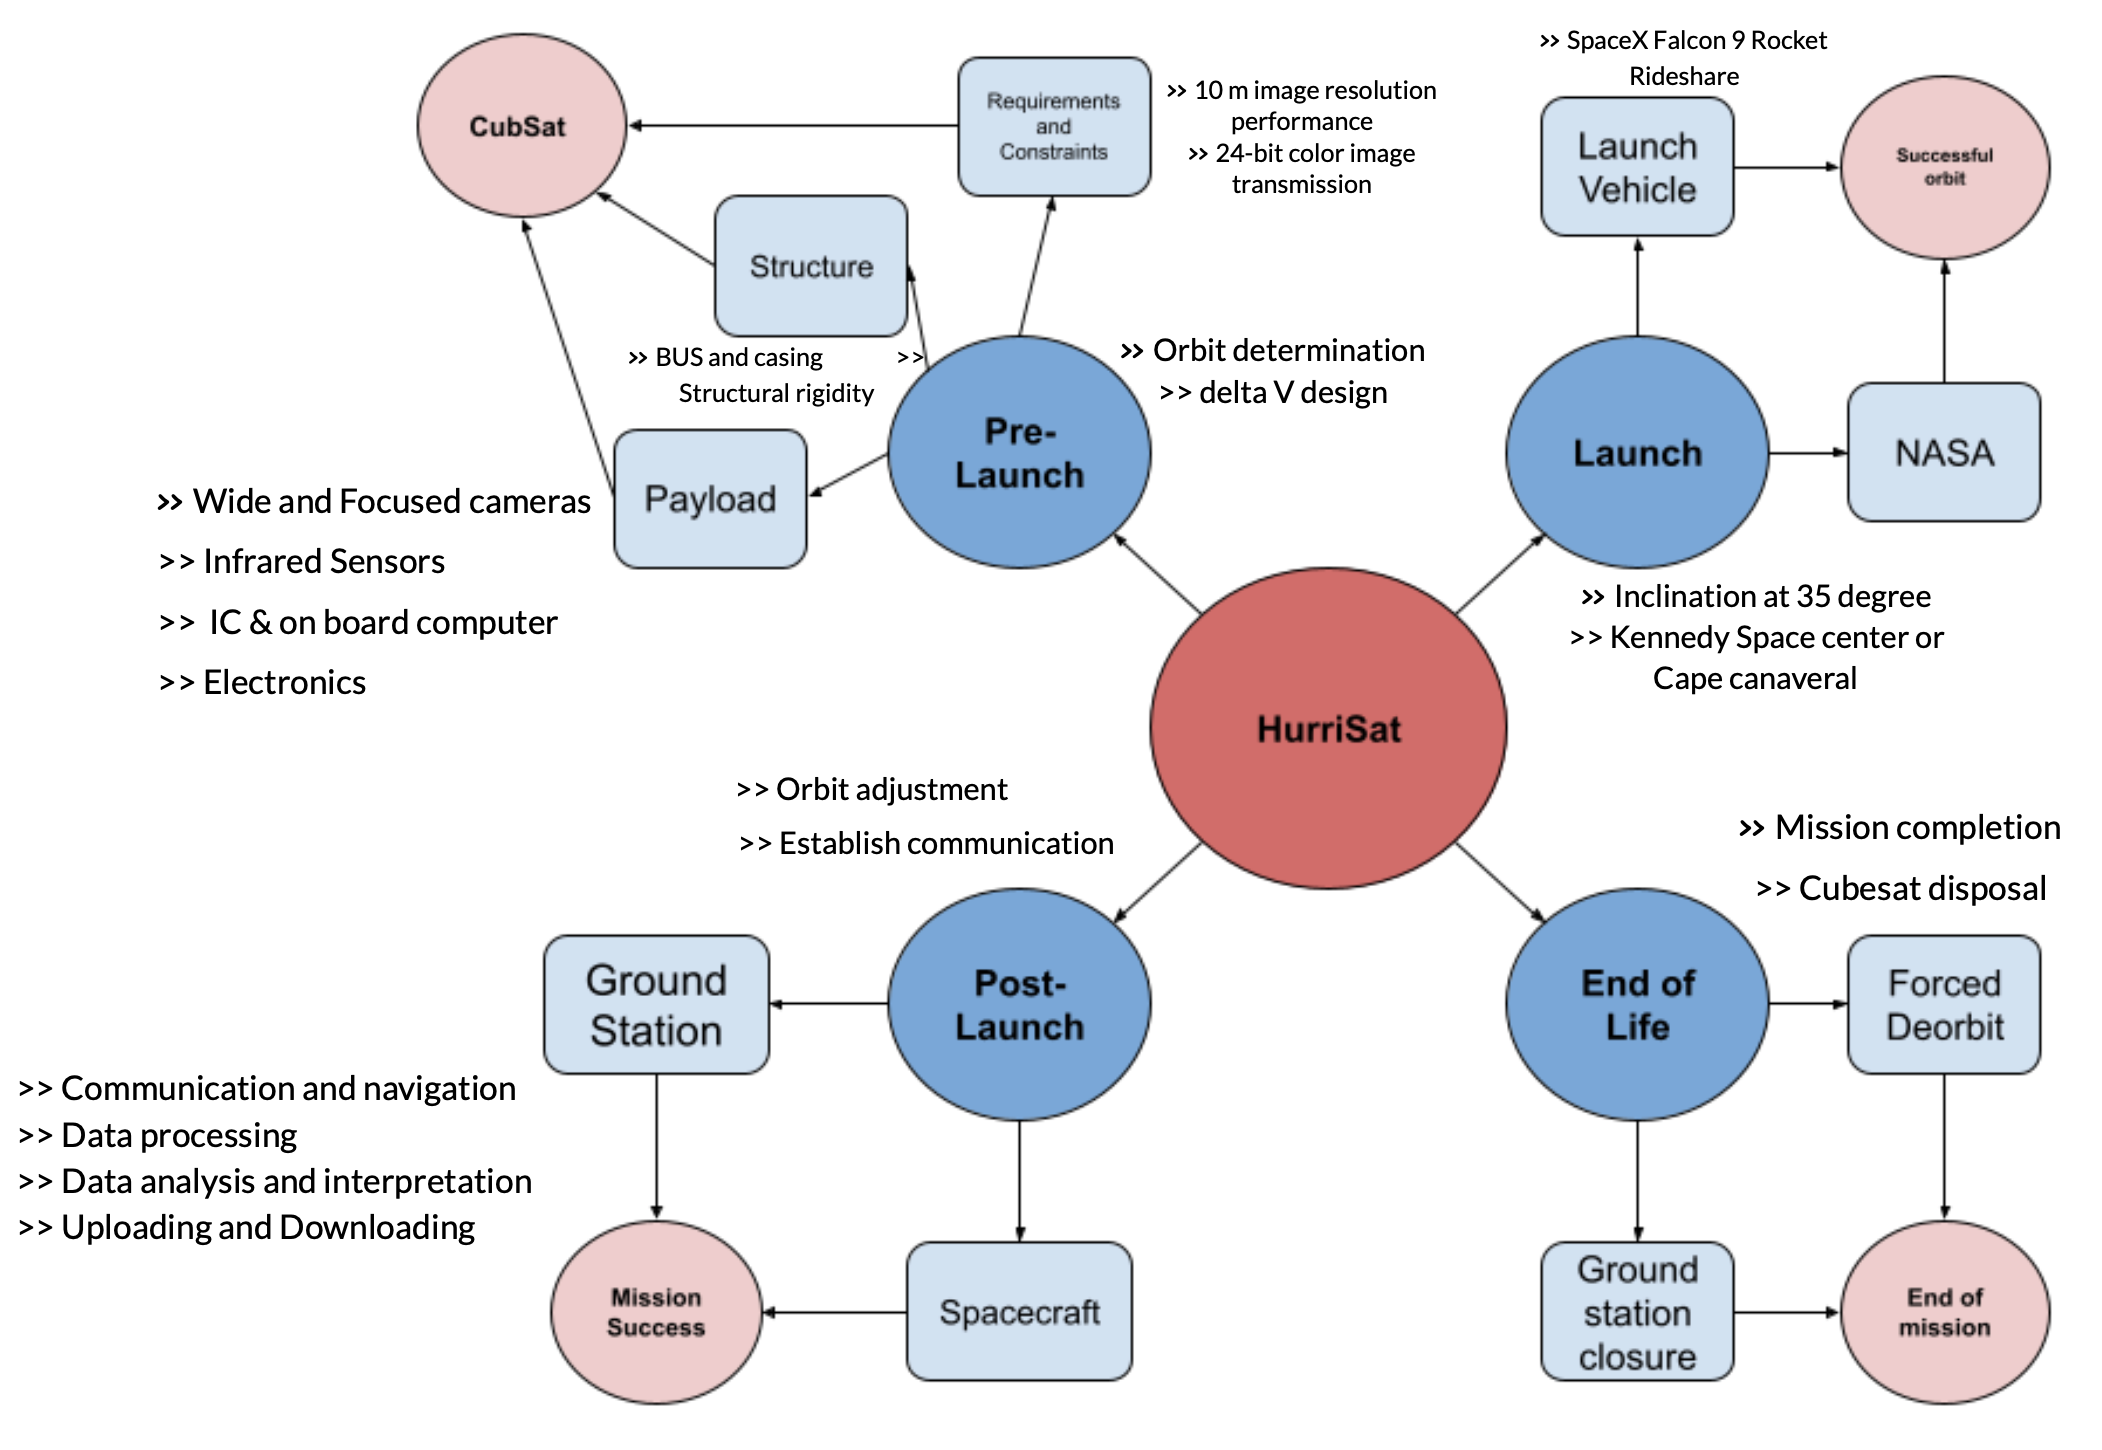
\includegraphics[width=\textwidth, frame,scale=0.9, keepaspectratio]{Images/march.png}
    \caption{Mission Architecture}
    \label{fig:march}
\end{figure}\\\\

\subsection{Mission Life}
The outline of the mission timeline for HurriSat is illustrated in Table \ref{Tab:clt}. The preliminary design Includes all the work completed within this report. Final Design will be the remaining design time used to complete design of the system and all supporting infrastructure to allow for execution of the strategic mission. Production and NASA integration will include the time to get approval from NASA, completion of all required documentations and licenses, and the construction of all required mission systems. Finally operation will include the time from launch until the eventual end of mission that will conclude with a force deorbit of the HurriSat system. In total, the HurriSat project is expected to have a total operation time of 17 years.

Additionally Figure \ref{fig:timelin} shows the life cycle block diagram. This diagram shows the expected timeline of HurriSat broken down into the Design, Production, Launch, Operation, and end of life phase. It also compares how the high level. Spacecraft (s/c), ground, and launch vehicles operate at the 5 phases of the cubesat's life cycle. \\
\FloatBarrier
\begin{table}[hbt!]
\centering
\caption{ Mission Life Summary}
\begin{tabular}{ll}
\rowcolor[HTML]{C0C0C0} 
Mission timeline                &   Expected                \\ \hline
Preliminary design              & 0.25 year         \\
Final design                    & 0.75 year         \\
Production and NASA integration & 1 year            \\
Operation                       & 15 years          \\ \hline
\textbf{Total}                  & \textbf{17 years}
\end{tabular}
\label{Tab:clt}
\end{table}

\begin{figure}[hbt!]
    \vspace{5mm}
    \centering
    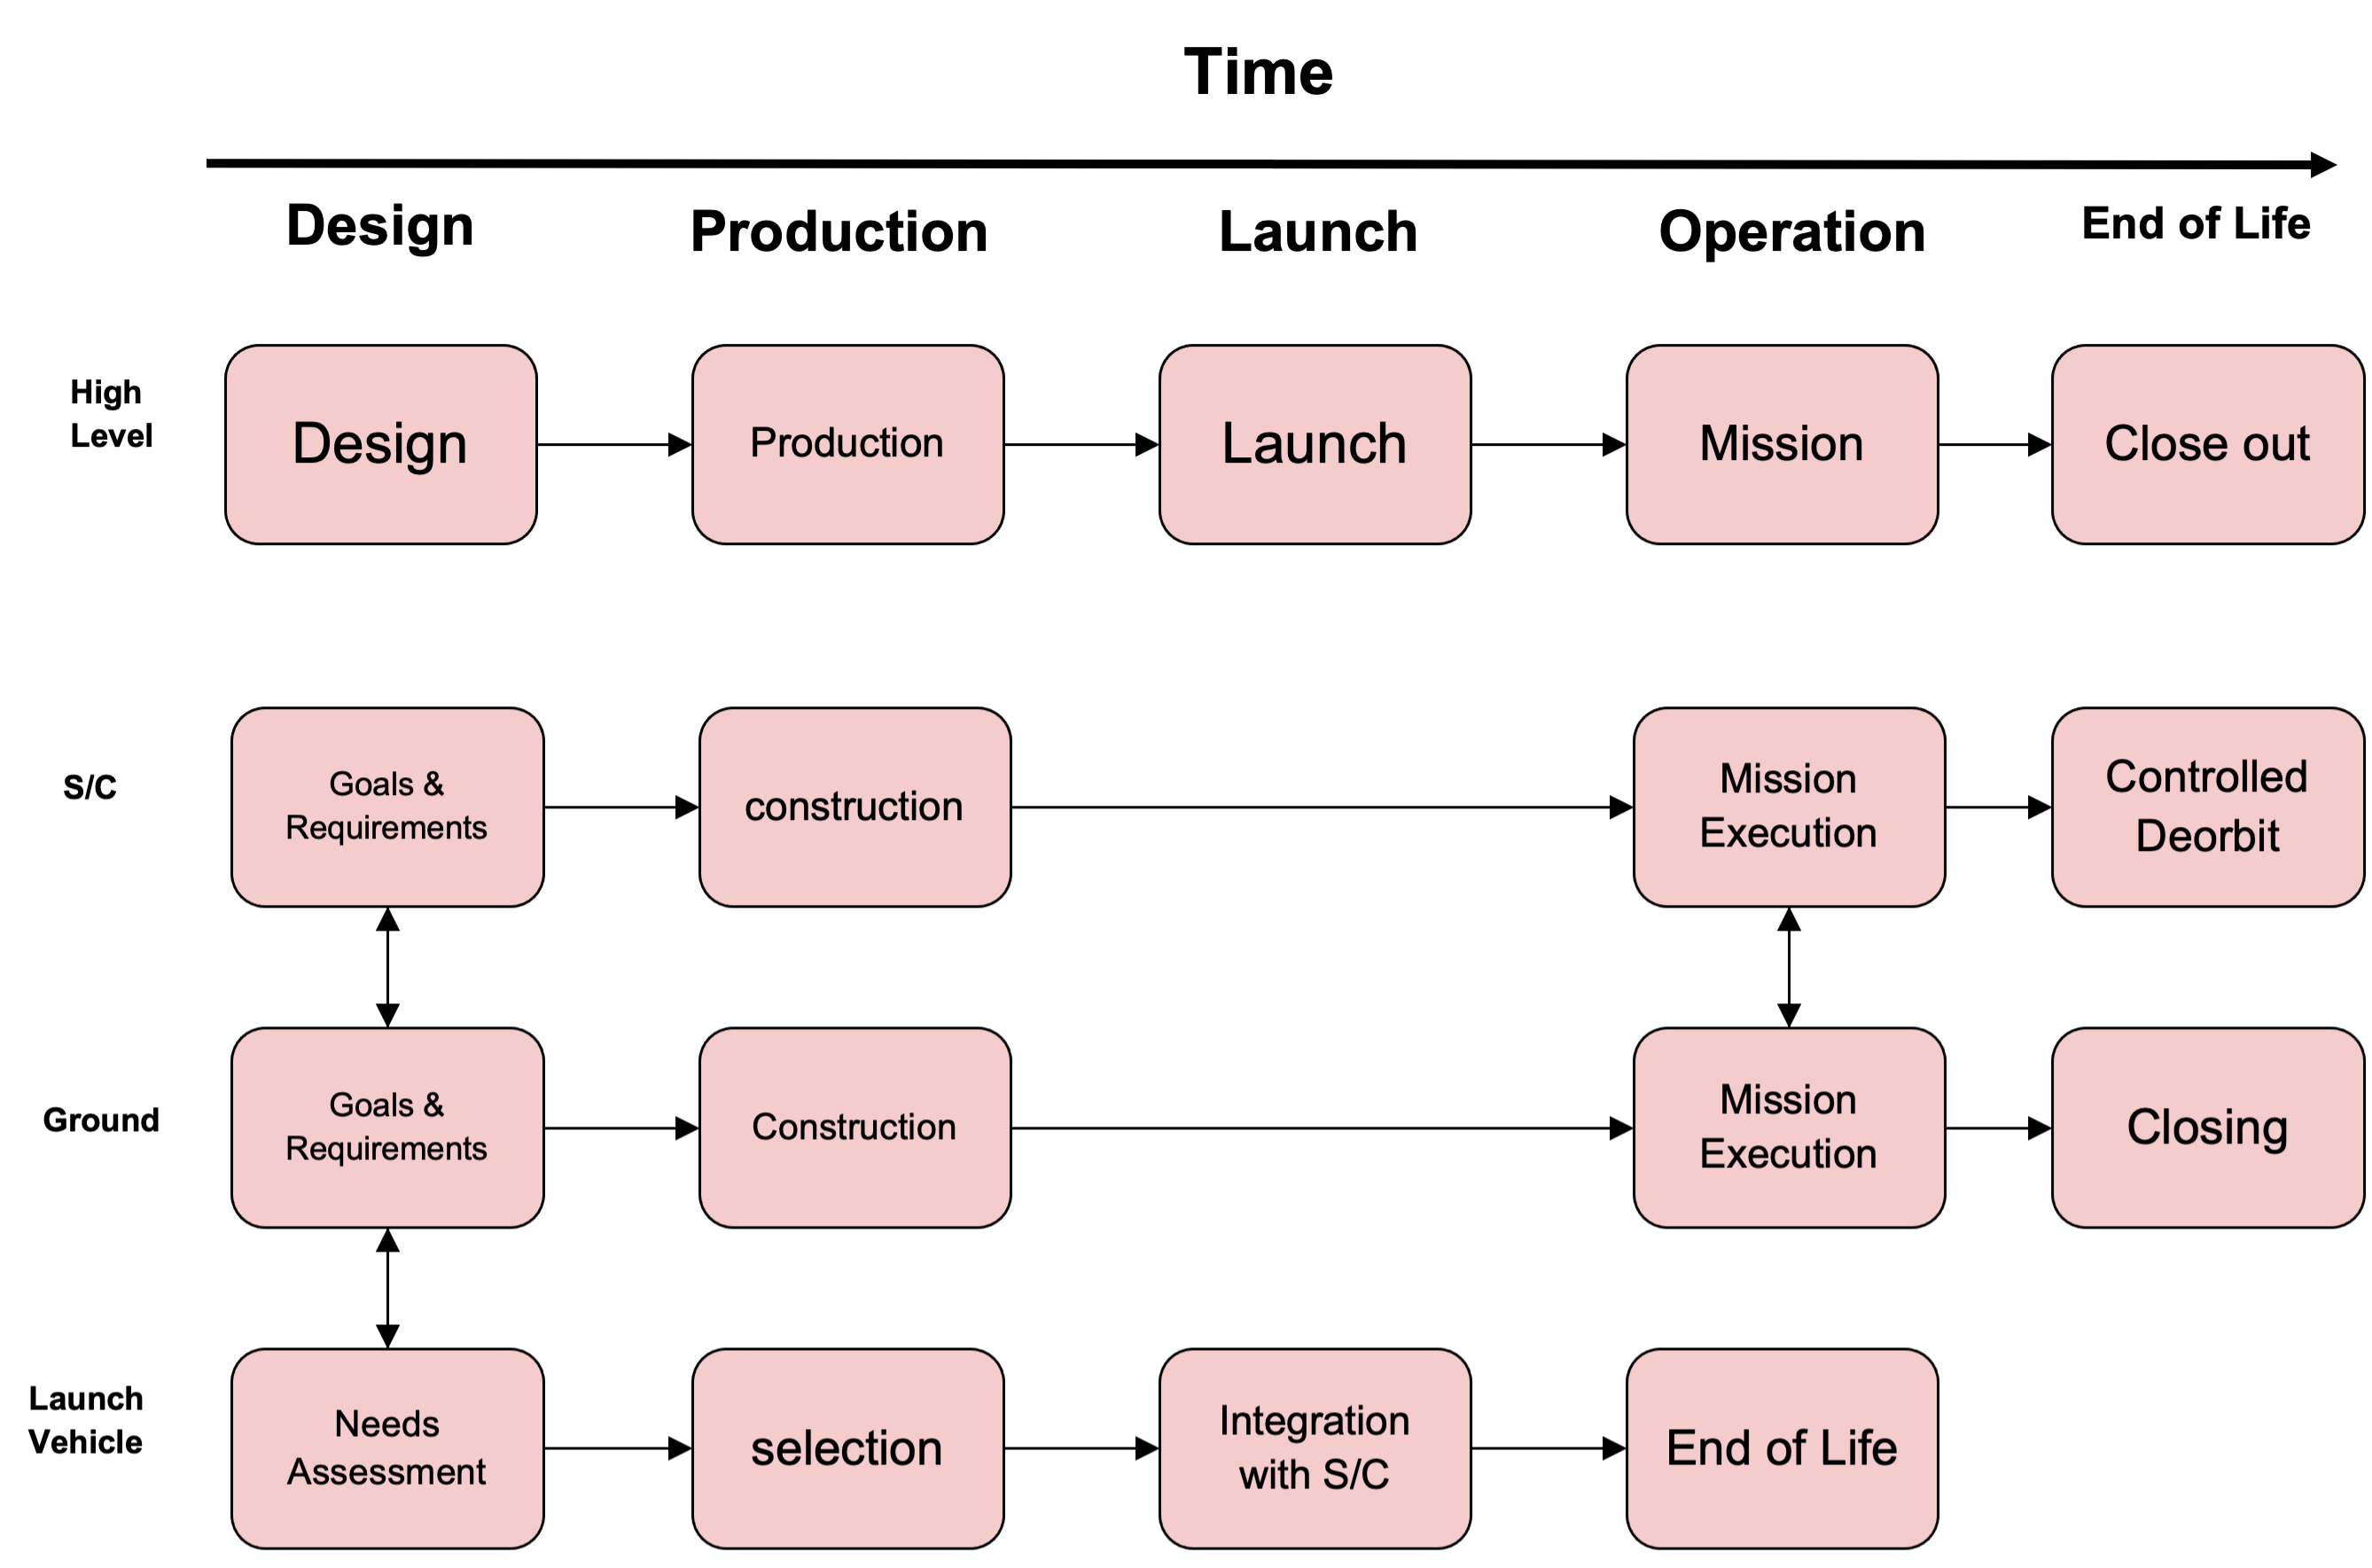
\includegraphics[keepaspectratio,width=\textwidth, frame, scale=0.8]{Images/timeline.png}
    \caption{HurriSat Timeline}
    \label{fig:timelin}
\end{figure}
\vspace{1cm}
Similarly Figure \ref{fig:diagram} is the sub-component functions block diagram. It is an interconnected functional overview for each subsystem in the cubesat. The main components in the payload (2 cameras) provide imagery function, while the on board computer process the data. The power is distributed as needed to all the componetes from the solar panels. The ADSC, propulsion all work together to help manage the cubesat's movement according to the ground stations needs.\\
\begin{figure}[hbt!]
    \vspace{5mm}
    \centering
    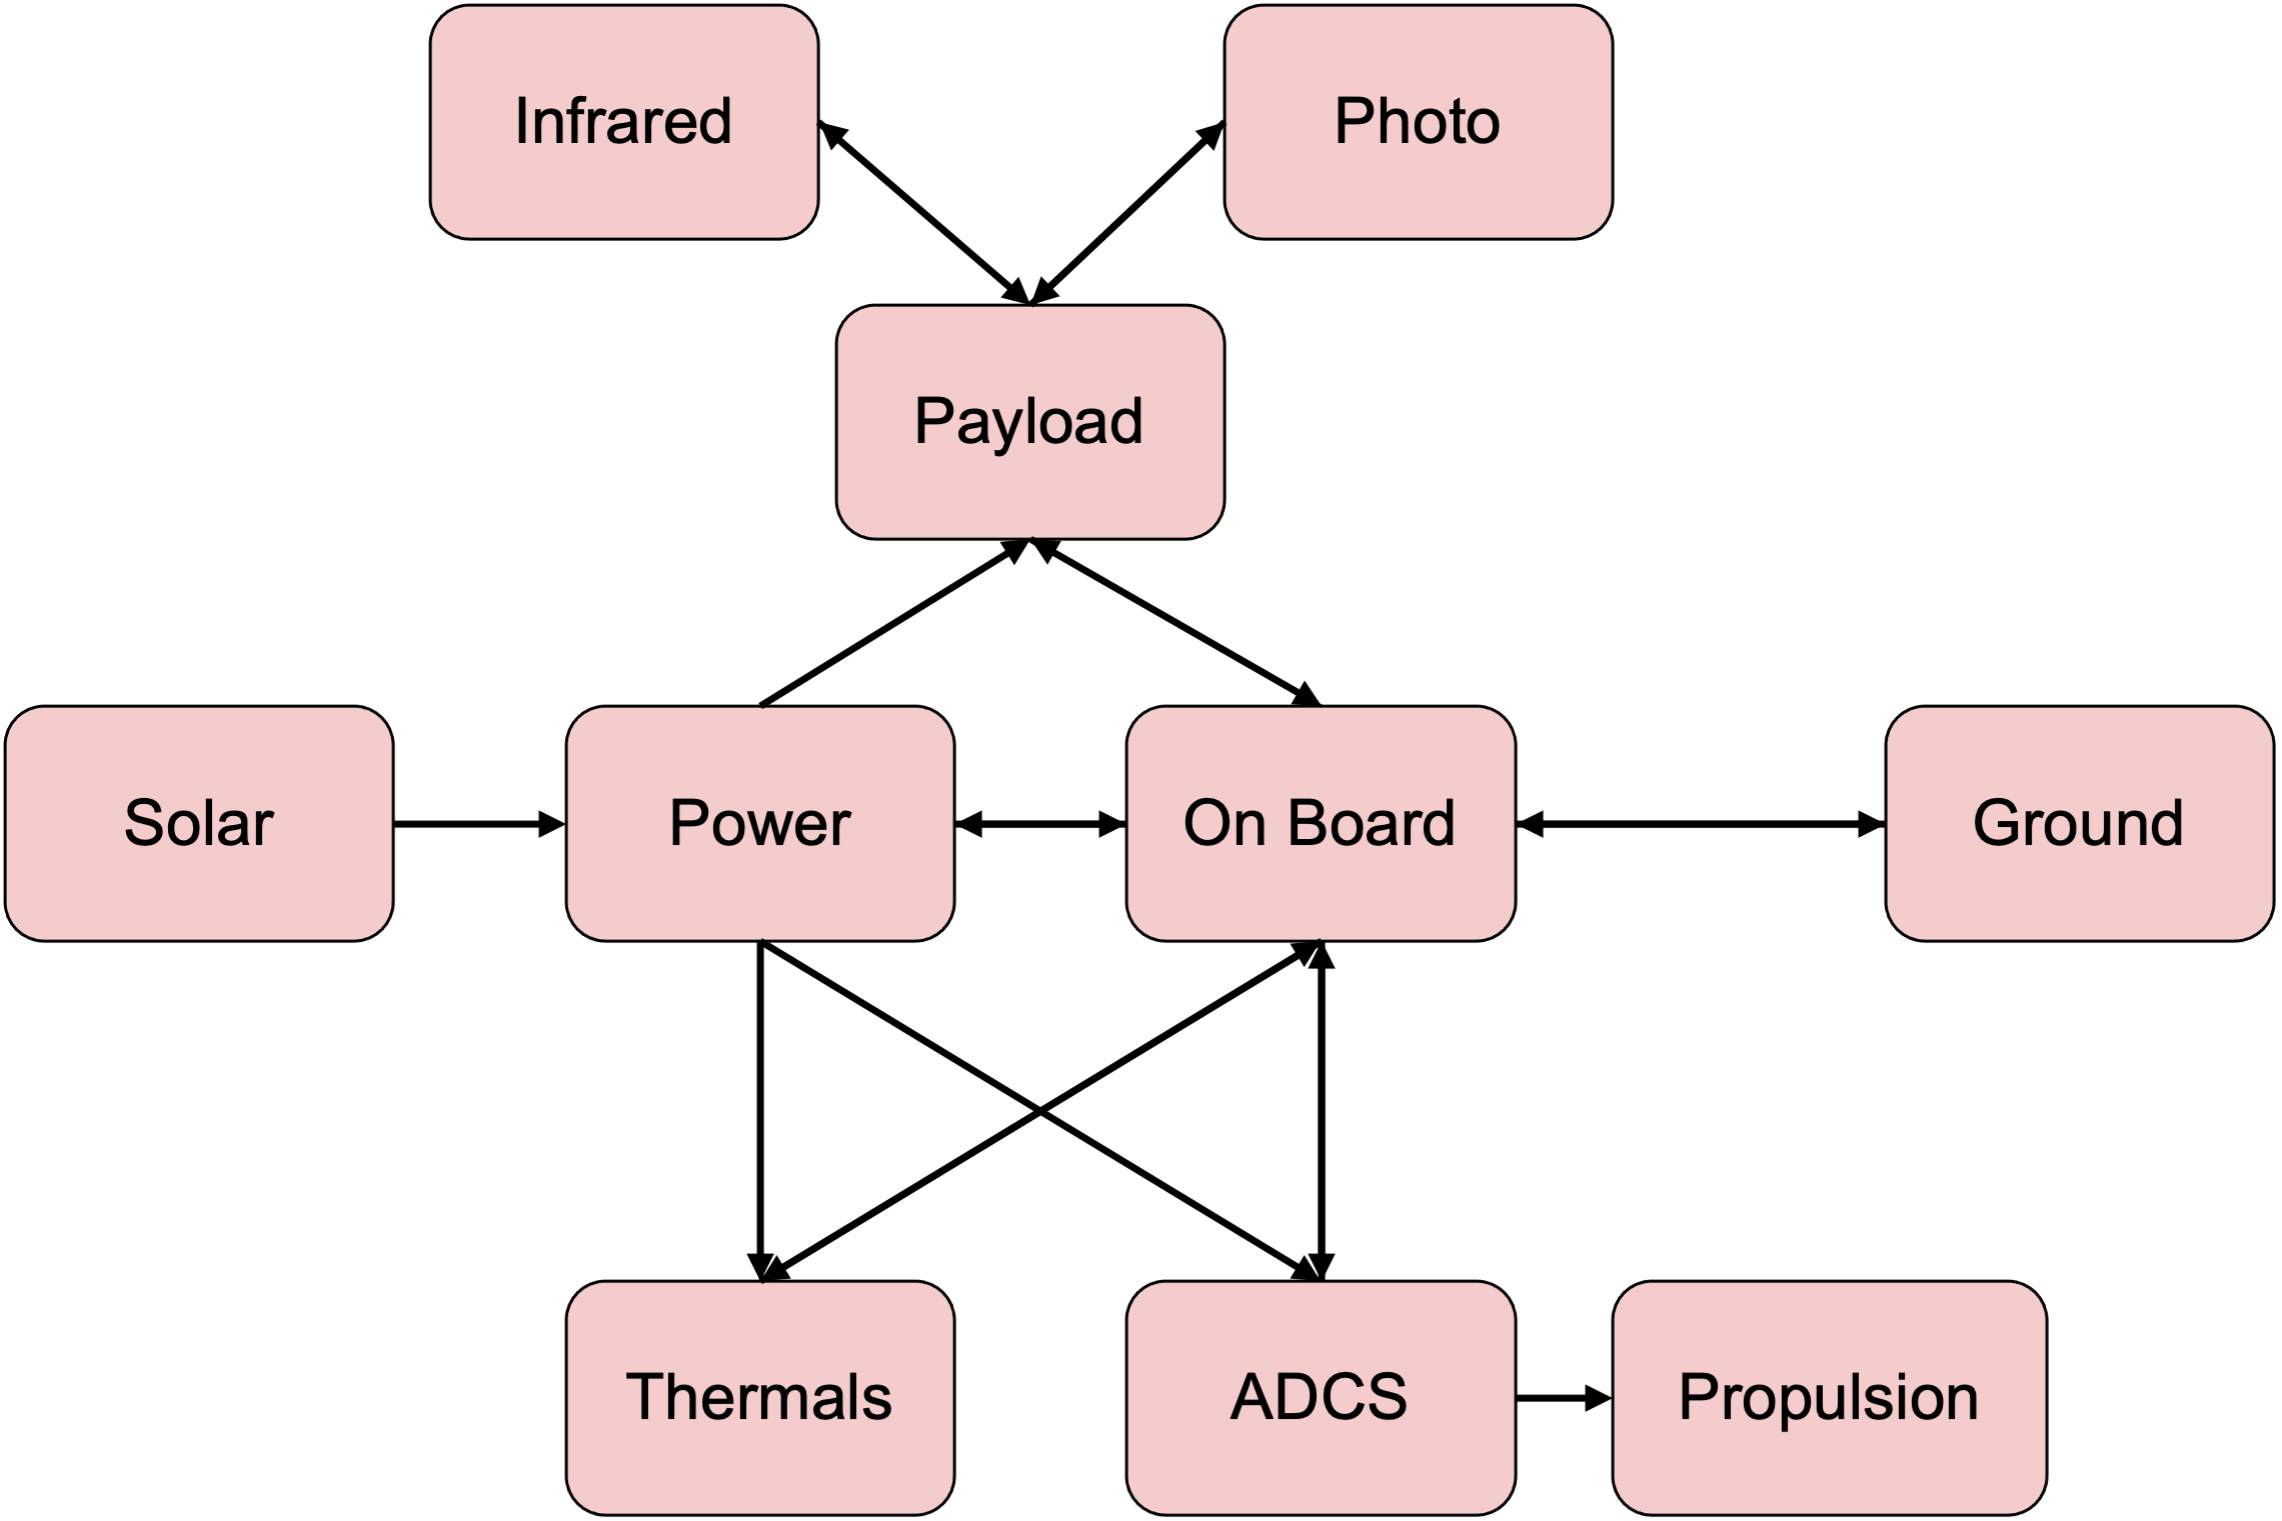
\includegraphics[keepaspectratio,width=\textwidth, frame, scale=0.8]{Images/diagram.png}
    \caption{Block Diagram}
    \label{fig:diagram}
\end{figure}
\FloatBarrier
\subsection{Launch Vehicle interface }
Considering all of the possible launch vehicles (see Table \ref{Tab:lvc}) available to NASA, the Falcon 9 Rocket (highlighted in red) is chosen as the best candidate. This is because SpaceX \cite{SpaceXFlacon-92021} is able to launch materials at a rate of \$1.1 million for up to 200kg per ride share. Additionally SpaceX has a frequent launch rate of roughly a launch every 4 months. HurriSat will integrate with the Falcon 9 rocket using SpaceX’s 157.5 cm diameter bolted interface. These factors will allow HurriSat to be launched in a timely manner at an affordable price.\\

\begin{table}[hbt!]
\centering
\caption{Launch Vehicles Compared}
\begin{tabular}{lllllll}
\rowcolor[HTML]{C0C0C0} 
\multicolumn{1}{c}{Launcher} &
  \multicolumn{1}{c}{Company} &
  \multicolumn{1}{c}{\begin{tabular}[c]{@{}c@{}}Launch Cost\\ (usd Million)\end{tabular}} &
  \multicolumn{1}{c}{\begin{tabular}[c]{@{}c@{}}Rocket Mass\\ (kg)\end{tabular}} &
  \multicolumn{1}{c}{Stages} &
  \multicolumn{1}{c}{\begin{tabular}[c]{@{}c@{}}Payload\\ (kg)\end{tabular}} &
  \multicolumn{1}{c}{\begin{tabular}[c]{@{}c@{}}Isp\\ (sec)\end{tabular}} \\ \hline
Minotaur       & Northrop Grumman       & \$50  & 73,000    & 4 & 1,458  & 286 \\
Delta II       & McDonnel Douglas       & \$51  & 286,000   & 3 & 6,140  & 319 \\
\rowcolor{red!20}Falcon 9       & SpaceX                 & \$67          & 549054    & 2 & 22800  & 275 \\
Falcon 9 Heavy & SpaceX                 & \$100 & 1,420,788 & 3 & 63,800 & 282 \\
Atlas V        & United Launch Alliance & \$125  & 590,000   & 2 & 18,850 & 280
\end{tabular}
\label{Tab:lvc}
\end{table}

\subsection{Orbital parameters}
The trade studies from initial report shows that GEO satellites are more than double the weight of LEO satellite.  This is typically because of that additional propellant they carry in order to transfer. The reason we chose a LEO orbit satellite is so that it's cheaper to operate and maintain at that altitude, cheaper to launch, light weight and utilizes that strong signal for communication. Hurrisat will be sharing a ride amongst other cubesats or shuttles heading to ISS or other missions. Typically it is cheaper (about \$1 million) compared to single launch at \$67 million. This incentives requires slecting best orbital parameters and launch sites. Launch sites for previous missions include Cape Canaveral Air Force Station,Pacific Missile Range Facility, Kennedy Space Center, Mojave Air and Space Port, and Rocket Lab Launch Complex \cite{NASA2022}. After careful observation and study \cite{Cipera2018} we have chosen the Kennedy Space center ($28.573^o$N and $80.649^o$W) in Florida as our launch site. It's also where SpaceX uses to launch our choice of rocket; the Falcon 9.

\subsubsection{Hohmann Transfer}
The Falcon 9 will be releasing it at around 400Km (closer to ISS altitude) \cite{NASA2017}. Since HurriSat will be sharing a launch vehicle amongst other it will need a Hohmann transfer.To transfer to its operational orbit of 800Km, it utilizes the propulsion and ADSC system. The Hohmann transfer values are shown in Table \ref{Tab:hoh}. These values are calculated with some marginal error for the actual weight and propulsion specific impulse provided by actual the manufacturer using a script, then simulated to STK. The orbital transfer is shown in Figure \ref{fig:hohfig}(a and b). \\
\FloatBarrier
\begin{table}[hbt!]
\centering
\caption{Transfer Values}
\begin{tabular}{ll}
\multicolumn{2}{l}{\cellcolor[HTML]{C0C0C0}\textbf{Initial Orbital Parameters}}       \\ \hline
Inclination         & 35 degrees      \\
Eccentricity        & 0 degrees       \\
Attitude            & 400 km          \\
\multicolumn{2}{l}{\cellcolor[HTML]{C0C0C0}\textbf{Hohmann Transfer: 400km to 800km}} \\ \hline
Delta V             & 0.217 km/s      \\
Transfer time       & 2900 s / 0.8 Hr \\
Eccentricity        & 0.514 degrees   \\
Inclination         & 35 degrees      \\
Radius of Periapsis & 6778.1 km       \\
Radius of Apoapsis  & 7175.1 km       \\
Semi-Major Axis     & 13956.3 km      \\
\multicolumn{2}{l}{\cellcolor[HTML]{C0C0C0}\textbf{Final Orbital Parameters}}         \\ \hline
Inclination         & 35 degrees      \\
Eccentricity        & 0 degrees       \\
Altitude            & 800 km         
\end{tabular}
\label{Tab:hoh}
\end{table}
\\
\begin{figure}
    \centering
    \subfloat[ Top View]{{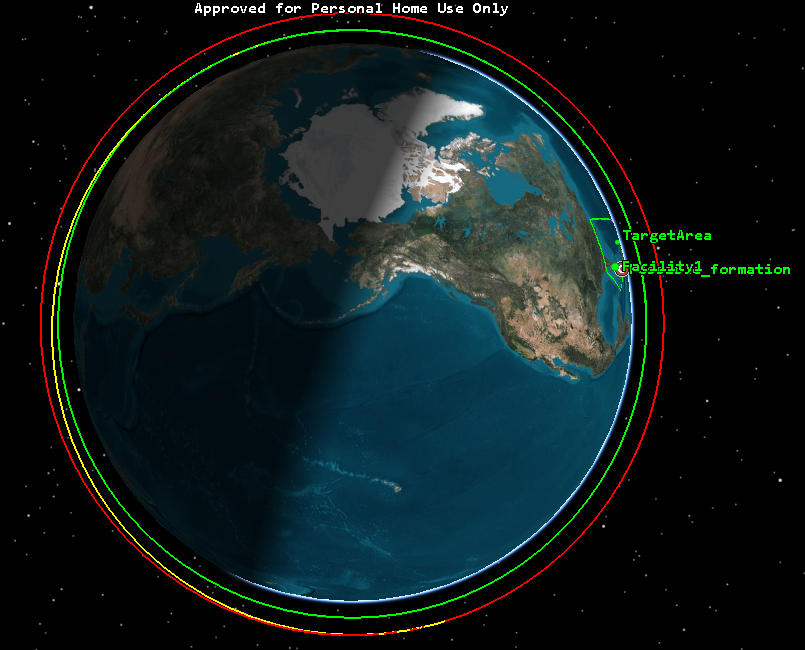
\includegraphics[width=8cm]{Images/t1.PNG} }}\label{fig:t1}
    \qquad
    \subfloat[Side View ]{{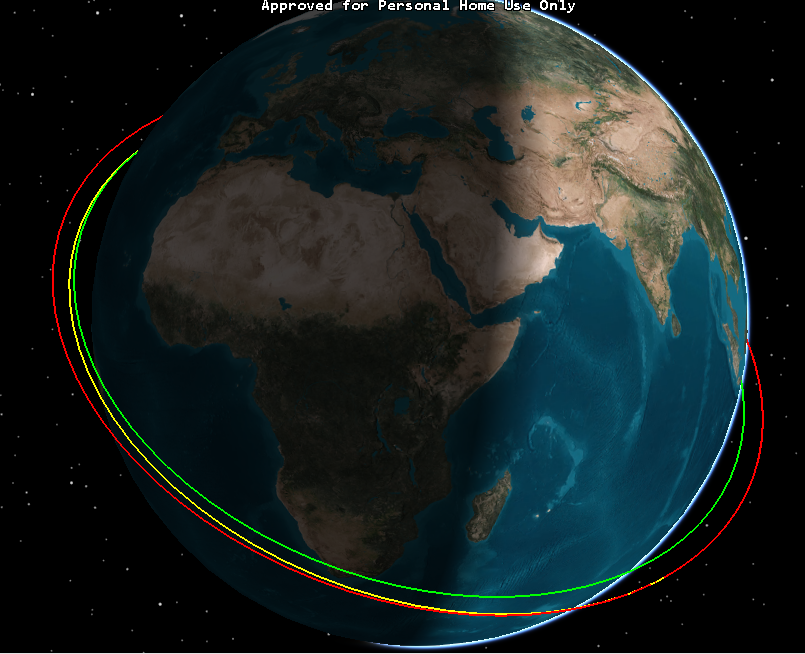
\includegraphics[width=8cm]{Images/t2.PNG} }}\label{fig:t2}
    \caption{Hohman Transfer simulated using STK}
    \label{fig:hohfig}
\end{figure}
\FloatBarrier
\subsection{Payload}
The payload is equipped with all the components needed for the mission. These components listed in Table \ref{Tab:pc} are selected specifically in order to meet the requirements. The payload comprises one visible spectrum image sensors behind a 2 setting variable zoom lens, one setting to detect possible hurricane formations alongside another to acquire detailed images, and an infrared spectrum sensor to provide hurricane characteristics. All fixed in orientation on the spacecraft. Camera and electronics weigh around $600 grams$ and the infrared sensor weighs around $45 grams$.\\

\begin{table}[hbt!]
\centering
\caption{Payload Characteristics}
\begin{tabular}{llll}
\rowcolor[HTML]{C0C0C0} 
Component      & Function                & Characteristics  & Requirements Met                                                       \\ \hline
IR camera      & Gather Atmospheric data & 640x512 pixels   & \begin{tabular}[c]{@{}l@{}}Temperature, \\ atmospheric readings\end{tabular} \\
Imaging sensor & capture images          & 4112x2248 pixels & \begin{tabular}[c]{@{}l@{}}Provide visible\\ spectrum images\end{tabular}    \\
Camera wide &
  \begin{tabular}[c]{@{}l@{}}Detect hurricane \\ formations\end{tabular} &
  2400x1300km; 548m/pixel &
  \begin{tabular}[c]{@{}l@{}}Yes, since 200m/pixel\\   \le 548m/pixel \end{tabular} \\
Camera narrow &
  \begin{tabular}[c]{@{}l@{}}Detailed hurricane \\ imaging\end{tabular} &
  26x14km coverage; 10m/pixel &
  \begin{tabular}[c]{@{}l@{}}Yes since 10m/pixel \\ \ge 6.5m/pixel \end{tabular} \\
  Antenna &  Transmission \& Comms          & 1 Mbps & \begin{tabular}[c]{@{}l@{}}Yes, can transmit 3\\ images per passs\end{tabular}    \\
  OBC ARM & Data Processing & 4112x2248 pixels & \begin{tabular}[c]{@{}l@{}}Provide visible\\ spectrum \end{tabular}    \\
\end{tabular}
\label{Tab:pc}
\end{table}

To achieve the ground coverage requirement of at least 10m/pixel the camera sensor has a resolution of $4112x2248pixels$ and a size of $3x2mm$ with a pixel size of $0.64μm$. The Spectral Camera's \ref{fig:cameras}(a) pixel size was selected based on the smallest available scale pixel technology and commercial availability. Narrow setting lens focal length was selected to equal $90mm$ to achieve a zoomed in image to sufficient ground resolution. With these specifications overall narrow camera lens ground resolution is 6.5m/pixel which exceeds the initial requirement of $10m/pixel$. Ground coverage is as required and equal to $26x14km$. The second lens setting is set at focal length of $1mm$ which results in a large half cone angle. This camera lens setting has the purpose of locating possible hurricane formations' location and relative speed. It has a ground resolution of $584m/pixel$. Area coverage on this setting is $2400x1312km$ which means that in most cases the satellite can cover the entire target area with a single pass.

The infrared camera in Figure \ref{fig:cameras}(b) is used to collect hurricane formation characteristics to the ground station. It's used to capture infrared pictures of could formation, temperature readings and other atmospheric readings with a configurable scan. It has a lower lens resolution compared to the visible spectrum cameras, however it is sufficient given that it only needs to give average temperature readings for a massive hurricane.\\


\begin{figure}
    \centering
    \subfloat[ Spectral Camera]{{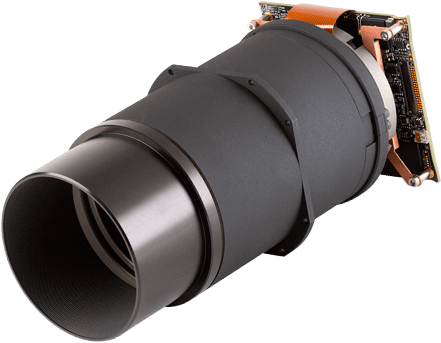
\includegraphics[width=8cm]{Images/sc.png} }}\label{fig:sc}
    \qquad
    \subfloat[Infrared Camera ]{{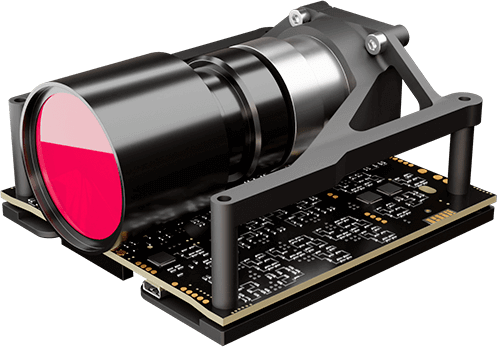
\includegraphics[width=8cm]{Images/ic.png} }}\label{fig:ic}
    \caption{Required Cameras}
    \label{fig:cameras}
\end{figure}


